\chapter{本地自适应差分隐私保护方法}

\label{ch3}

\section{引言}
与传统的集中式深度学习相比,联邦学习通过分布式训练在一定程度上缓解了隐私泄漏的问题。然而,许多研究表明,在训练过程中,本地设备与中央服务器之间的通信信道和传递的模型参数都有可能成为第三方窃取敏感信息的途径,联邦学习的框架仍然存在本地训练数据泄漏等隐私威胁\upcite{ref48}。深度学习技术可以“记忆”模型中的训练数据信息,在这种情况下,敌方一旦通过白盒推理攻击或者黑盒推理攻击访问模型,就可以推演出客户端本地的训练数据。

在第二章的基础知识中我们介绍了联邦学习模型的整体流程,联邦学习模型的优化问题可以概括为ERM(经验风险最小化)问题\upcite{ref40}:
\begin{equation}\label{eq:ERM}
\arg \min _{\theta \in \mathcal{C}}\left(F(\theta):=\frac{1}{m} \sum_{i=1}^{m} F_{i}(\theta)\right)
\end{equation}

通过优化ERM函数间接优化模型参数,使模型的实际输出与预测值更加接近,模型的准确率越高。从隐私保护的角度讲,我们只要截断了从原始输入到输出,在其中加入一道隐私保护屏障,具体在哪一步截断则对应于不同的方法。差分隐私保护机器学习的方法具体有以下几种:
\begin{itemize}
	\item \textbf{输入扰动:} 输入扰动是在获取的训练数据上直接添加噪声,之后的模型训练和优化都是基于加躁后的训练数据\upcite{ref37}\upcite{ref38}\upcite{ref39}。
	\item \textbf{输出扰动:} 输出扰动沿袭了拉普拉斯机制最简单的思路,即考虑函数输出的敏感度来添加噪声,那么在ERM公式中我们只需要考虑argmin函数输出的敏感度,基于这个敏感度来添加拉普拉斯噪声即可得到一个简单的满足差分隐私的ERM方法\upcite{ref36}。
	\item \textbf{梯度扰动:} 梯度扰动是在执行最小化损失函数的过程中,设计满足差分隐私的算法。
	\item \textbf{目标扰动:} 目标扰动是在模型的目标函数中添加一个随机量,以使得最终模型的输出满足随机性。
\end{itemize}

基于输入的扰动和输出的扰动基本可以视为一个黑匣子模型,简单直接。但是这种添加噪声的方式无法对训练过程中数据的相互依赖性和输出有效性作出有用的、紧密的描述。在输入数据中加入过多的噪声,可能会影响模型训练的收敛性。在输出参数中加入过于保守的噪声,也就是根据最坏的攻击情况去添加噪声,可能会影响模型的实用性。

当前在深度学习模型中应用差分隐私的主流方案是在模型的梯度上添加噪声,方案的目标是在满足差分隐私的条件下,实现整体模型的最优可用性。Song等人\upcite{ref47}提出了一个$\left(\epsilon_{c}+\epsilon_{d}\right)$-差分隐私版本的随机梯度下降算法。在本地模型的每一次迭代过程中,对梯度添加高斯噪声,并通过差分隐私的组合性和隐私放大效果,得到完全隐私损失的上界。

与SGD 相比,差分隐私随机梯度下降 (DP-SGD) 严重降低了训练模型的效用。 如图所示,当差分隐私隐私提供的隐私强度增加时,MNIST数据集上逻辑回归的训练和验证的损失率迅速增加。由DP-SGD训练的卷积神经网络(CNN)的测试精度比MNIST 上的非差分隐私网络低得多。Goodfellow\upcite{ref64}提出了$\ell_{2}$范式梯度裁剪的方式以限制函数敏感度,并设计了“Moments Accountant”(MA)来计算更准确的隐私预算估计。

然而,在传统的基于差分隐私的联邦学习框架中,数据管理者倾向于给每个用户的数据以相同的隐私预算,同样的隐私预算忽略了用户之间的差异。有些用户希望有更好的隐私保护。而有些用户对某些数据的隐私不敏感。在这种情况下,由于联邦学习模型是分布式结构,从一个大数据库到许多小数据库,所以对于每个用户来说。他们只需要关心他们自己的隐私。他们可以设置不同的隐私预算方案,而不是传统的统一分配,然后在最坏的的情况下注入噪音。而基于梯度扰动的方法的问题在于它们的迭代性质会导致隐私预算的飙升。因此,当前的主要挑战是设计一种新型的满足差分隐私的扰动算法,既能保证模型的效用性,并且维持较高的计算效率。

本文采用一种更加复杂的方法来分析训练过程中训练数据对模型输出的贡献比率,然后根据每一层神经网络对模型输出的贡献率,在梯度上根据贡献比率添加对应的噪声量,在进行梯度下降之前,根据神经网络的层次对梯度进行自适应的裁剪,保证模型的收敛率。我们的方法不仅产生了在模型精度方面最接近非差分隐私的模型,而且还降低了隐私预算的成本。

\section{模型设计}

\subsection{模型概览}
传统的联邦学习中使用差分隐私的主要流程如下所示:
\begin{itemize}
\item \textbf{本地计算:}
客户端 $\mathrm{i}$ 根据本地数据库 $\mathcal{D}_{\mathrm{i}}$ 和接受的服务器的全局模型 $\mathrm{w}_{\mathrm{G}}^{\mathrm{t}}$ 作为本地的参数,即 $\mathrm{w}_{\mathrm{i}}^{\mathrm{t}}=\mathrm{w}_{\mathrm{G}}^{\mathrm{t}}$, 采用梯度下降策略进行本地模型训练得到 $\mathrm{w}_{\mathrm{i}}^{\mathrm{t}+1} \quad(\mathrm{t}$ 表示当前通信回合) 。

\item \textbf{模型扰动:}
每个客户端产生一个随机噪音 $\mathrm{n},\mathrm{n}$ 是符合高斯分布的,使用 $\overline{\mathbf{w}_{\mathrm{i}}}^{\mathrm{t}+1}=\mathrm{w}_{\mathrm{i}}^{\mathrm{t}+1}+\mathrm{n}$ 扰动本地模型 (这里注意w是一个矩阵,n表示对矩阵的每一个元素添加噪音)。

\item \textbf{模型聚合:}
服务器使用参数聚合算法聚合从客户端收到的 $\overline{\mathrm{w}}_{\mathrm{i}} \mathrm{t}+1$ ,得到新的全局模型参数 $\mathrm{w}_{\mathrm{G}}^{\mathrm{t}+1}$, 也就是扰动过的模型参数。

\item \textbf{模型广播:}
服务器将新的模型参数广播给每个客户端。

\item \textbf{全局收敛:}
重复步骤(1)-(4)直至全局模型收敛。
\end{itemize}

本文的模型主要针对本地设备的模型训练添加自适应的噪声和梯度裁剪算法,保证中央服务器接收到的满足$\epsilon$-差分隐私的权重,从而防止模型反演攻击、模型重建攻击、成员推理攻击等。

在本文中,我们认为中央参数服务器是半可信的(Honest but Curious, HbC),一个"诚实但好奇"的实体。也就是说,服务器将遵循与所有用户的协议。然而,通过利用通信信道访问用户梯度的便利,它也试图在训练过程中反推出关于客户端的额外的信息。出于这个原因,我们的提出的自适应加噪机制目的是保护发送到服务器的本地梯度不被推断出任何关于用户的本地训练样本信息,并且尽量维持原有模型的精度。为实现相同的效用保证,我们算法的梯度复杂度(即计算的随机梯度总数)为$O\left(n^{3 / 2}\right)$,比之前的最佳结果高出$\Theta\left(n^{1 / 2}\right)$。 之后我们在MNIST和FICAR-10数据集上进行实验,评估我们提出的方法,并与前人的四种差分隐私保护方案进行对比,发现我们的方法不仅产生了在模型精度方面最接近非差分隐私的模型,而且还降低了隐私预算。并且,我们针对添加本地自适应差分隐私方案的模型进行成员推理攻击,评估了该方案的隐私保护效应。

总的来说,本章提出的隐私保护方案是基于本地客户端的本地数据维度,从以下两个方面展开研究:
\begin{enumerate}
\item [(1)] 通过在本地模型训练的梯度下降算法过程中针对不同层的贡献比自适应添加高斯噪声。
\item [(2)] 根据训练轮数和层间贡献率对梯度进行自适应裁剪。
\end{enumerate}

\subsection{自适应噪声添加算法}
在第二章我们详细介绍了联邦学习的流程和神经网络的结构,每个用户在本地设备在私有数据集上进行训练,得到本地模型的输出。本地训练的流程如图\ref{fig:神经网络的前向传播和反向传播流程图}所示,神经网络中前向传播算法的第一步在输入层。我们使用前馈神经网络接收输入的$x$运行前向传播算法,得到预测值,然后通过反向传播算法不断调整参数使与预测值和真实值之间的误差降低。Bach等人提出了针对神经网络的逐层关联传播算法\upcite{ref65},它允许分解深度神经网络的预测值,我们利用该算法将神经网络的输出值按层进行分解,得到每层的属性值对于模型输出的贡献比,然后根据属性的贡献率,在梯度下降的过程中添加对应比的高斯噪声。

\begin{figure}[!hbt]
\centering
	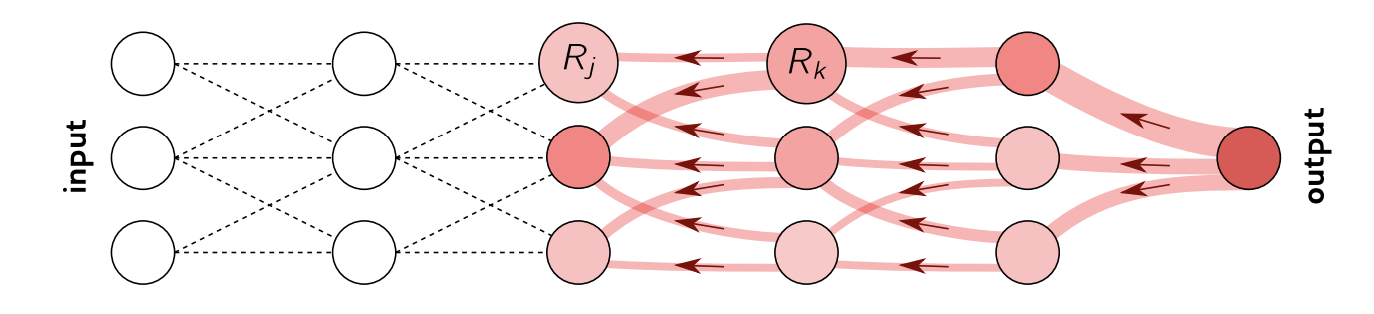
\includegraphics[scale=0.45]{fig2/C3/逐层关联传播算法}%联邦学习的系统架构
	\caption{神经网络的前向传播和反向传播流程图}
	\label{fig:神经网络的前向传播和反向传播流程图}	
\end{figure}

在逐层关联传播算法中,根据神经网络的结构自后向前计算归因值,也称为相关性分数。对于卷积神经网络等网络结构,从输出层开始根据反向传播算法计算归因分数,输出层的归因分数通常作为输出层的预激活值,在反向传播过程中,每一层的所有神经元的归因分数总和是恒定。

在卷积神经网络结构中,每个隐藏神经元的转化过程表示为$y=a(\mathbf{x} * \omega+b)$,其中$\mathbf{x}$代表输入向量,$y$是输出,$b$和$\omega$分别代表{}偏置项和权重矩阵。$a()$是一个激活函数,用于结合线性变换和非线性变换。

由于神经网络的结构,上一层的输出是下一层的输入,由此我们可以得出,原始的训练数据只被第一个隐藏层的线性变换所利用。直白地说,为了得到一个具有隐私保护的学习模型,我们可以在第一个隐藏层的数据中注入噪声。正如Phan等人\upcite{ref36}提到的,对于线性变换有一种传统的方法,即向原始数据注入具有相同隐私预算的噪声,但是这容易导致隐私预算增加,并且使原始数据失真过多。因此,本文提出一种自适应噪声添加算法,针对每个梯度计算其贡献值,根据属性对于模型输出的贡献率添加对应比例的高斯噪声。

令$C_{a_{i}}^{l_{k}}\left(x_{i}\right)$表示第$k$层的神经元 $a_{i}$,"$\leftarrow$"表示神经网络每一层之间的连接关系。"$l_{k} \leftarrow l_{k+1}$" 是指深度神经网络中第k层和第k+1层之间相邻层的连接关系。对于模型输出的贡献率,根据神经网络相邻层间的线形关系,那么神经元$a_{i}$的贡献率即为与之相邻的第$k+1$层的神经元的贡献率之和:
$$
C_{a_{i}}^{l_{k}}\left(x_{i}\right)=\sum_{a_{j} \in l_{k+1}} C_{a_{i} \leftarrow a_{j}}^{l_{k} \leftarrow l_{k+1}}\left(x_{i}\right)
$$

当第k层为输出层时,我们有:
\begin{equation}
C_{a_{i}}^{l_{k}}\left(x_{i}\right)=f\left(x_{i}, \omega_{i}^{r}\right)
\end{equation}

根据矩阵层之间的线性相关性,神经元$a_{i}$在第k层的贡献$C_{a_{i}}^{l_{k}}\left(x_{i}\right)$等于连接到神经元$a_{i}$的相邻层的贡献之和:
\begin{equation}\label{eq:层间传播1}
C_{a_{i}}^{l_{k}}\left(x_{i}\right)=\sum_{a_{j} \in l_{k+1}} C_{a_{i} \leftarrow a_{j}}^{l_{k} \leftarrow l_{k+1}}\left(x_{i}\right)
\end{equation}

因此,位于输出层的神经元$a_{j}$的贡献等于模型的输出。第k-1层的神经元$a_{j}$对于第k层的神经元的贡献$C_{a_{i} \leftarrow a_{j}}^{l_{k-1} \leftarrow l_{k}}\left(x_{i}\right)$等于:
\begin{equation}
C_{a_{i} \leftarrow a_{j}}^{l_{k-1} \leftarrow l_{k}}\left(x_{i}\right)=\left\{\begin{array}{cc}\frac{a_{i} w_{i, j}}{\sum_{a_{i} \in l_{k-1} a_{i} w_{i, j}}} C_{a_{j}}^{l_{k}}\left(x_{i}\right) & \sum_{a_{i} \in l_{k-1}} a_{i} w_{i, j} \neq 0 \\ \mu & \sum_{a_{i} \in l_{k-1}} a_{i} w_{i, j}=0\end{array}\right.
\end{equation}

其中$\mu$是一个无限接近于零,但大于零的数字。从上述公式中,我们可以认为每一层的贡献是相等的,而且贡献是逐层传递的。根据以上公式的推导,我们能得到神经网络模型中每一层以及每个神经元的贡献值。那么模型的输出可以表示为层神经元贡献值的累加:
$$
\begin{aligned}
\sum f\left(x_{i}, \omega_{i}^{r}\right) &=C_{a_{8}}^{l_{3}}\left(x_{i}\right)+C_{a_{9}}^{l_{3}}\left(x_{i}\right)\\
&+C_{a_{4}}^{l_{2}}\left(x_{i}\right)+C_{a_{5}}^{l_{2}}\left(x_{i}\right)+C_{a_{6}}^{l_{2}}\left(x_{i}\right)+C_{a_{7}}^{l_{2}}\left(x_{i}\right)\\
&+C_{a_{1}}^{l_{1}}\left(x_{i}\right)+C_{a_{2}}^{l_{1}}\left(x_{i}\right)+C_{a_{3}}^{l_{1}}\left(x_{i}\right)
\end{aligned}
$$

通过从数据元组中提取同一属性的贡献,我们可以计算出每个属性类对模型输出的平均贡献:
\begin{equation}\label{eq:属性添加自适应扰动}
C_{j}\left(x_{i}\right)=\frac{1}{n} \sum_{i=1}^{n} C_{x_{i, j}}\left(x_{i}\right), j \in[1, u]
\end{equation}

然后,我们引入了两个调整参数$f$和$p$。其中,$f$代表一个阈值,用于决定属性对模型结果输出的归因分数是高还是低,其值由联邦学习中的本地用户自己定义,即贡献超过阈值$f$的梯度对输出的贡献更大,我们向所有这些梯度注入自适应拉普拉斯噪声。当归隐分数低于阈值$f$时,对这些梯度进行概率选择。也就是说,我们抛弃概率为$1-p$的原始数据,并对一些概率为$p$的梯度注入自适应高斯噪声。该公式如下:
\begin{equation}\label{eq:神经网络加噪}
\tilde{x}_{i, j}=\left\{\begin{array}{ll}
\ddot{x}_{i, j} & \beta \geq f \\
\bar{x}_{i, j} & \beta<f
\end{array}\right.
\end{equation}

其中$\beta$代表该层神经元的归因分数:$\beta=\frac{\left|\ddot{C}_{j}\right|}{\sum_{j=1}^{u}\left|\ddot{C}_{j}\right|}$,当$\beta<f$时,我们有:
\begin{equation}\label{eq:神经网络加噪2}
\bar{x}_{i, j}=\left\{\begin{array}{l}
\ddot{x}_{i, j} \text { with probability } p \\
x_{i, j} \text { with probability } 1-p
\end{array}\right.
\end{equation}

在此方案中,隐私预算$\epsilon_{l}$是根据各自的归因分数按比例分配给每个梯度:$\sigma$=$\sigma_{j}=\frac{u *\left|\ddot{C}_{j}\right|}{\sum_{j=1}^{u}\left|\ddot{C}_{j}\right|} * \sigma_{l}$,自适应高斯噪声按以下方式注入梯度中:
\begin{equation}\label{eq:神经网络加噪3}
x_{i, j}^{\prime}=x_{i, j}+\frac{1}{\left|D_{i}^{t}\right|}\mathcal{N}\left(0, S_{f}^{2} \cdot \sigma^{2}\right)
\end{equation}

在不失一般性的情况下,调整因子$f$和$p$的值与系统的准确性和隐私水平有关。即$f$越小,$p$越大,代表越高的隐私保护水平,模型准确性越低,反之亦然。算法\ref{自适应高斯噪声算法}详细描述了自适应高斯噪声算法,我们将层间依赖算法于随机梯度下降算法相结合,关键的步骤包括:计算梯度以及归因分数,根据归因分数分配相应的隐私预算,在梯度上添加高斯噪声,最后进行梯度下降。\\

\begin{algorithm}[!htb]
	\caption{自适应高斯噪声算法}
	\label{自适应高斯噪声算法}
	\begin{algorithmic}[1]
		\footnotesize
		\STATE \textbf{输入:} 数据集 $\left\{x_{1}, \ldots, x_{N}\right\}$,损失函数$\mathcal{L}(\theta)=$ $\frac{1}{N} \sum_{i} \mathcal{L}\left(\theta, x_{i}\right)$,学习率$\eta_{t}$, 隐私预算$\sigma$, 批大小$L$
		\STATE 初始化:模型权重$\theta_{0}$
		\FOR{ $t \in[T]$}
			\STATE 以概率$L / N$随机采样一批数据集$L_{t}$
			\STATE 计算梯度:$\mathbf{g}_{t}\left(x_{i}\right) \leftarrow \nabla_{\theta_{t}} \mathcal{L}\left(\theta_{t}, x_{i}\right)$
			\STATE 计算梯度的贡献率:$\beta=\frac{\left|\ddot{C}_{j}\right|}{\sum_{j=1}^{u}\left|\ddot{C}_{j}\right|}$
			\STATE 根据贡献率分配相应的隐私预算:$\sigma==\frac{u *\left|\ddot{C}_{j}\right|}{\sum_{j=1}^{u}\left|\ddot{C}_{j}\right|} * \sigma_{l}$
			\STATE 添加高斯噪声:$\tilde{\mathbf{g}}_{t} \leftarrow \frac{1}{L} \sum_{i}\left(\overline{\mathbf{g}}_{t}\left(x_{i}\right)+\frac{1}{\left|D_{i}^{t}\right|}\mathcal{N}\left(0, S_{f}^{2} \cdot \sigma^{2}\right)\right)$
			\STATE 梯度下降:$\theta_{t+1} \leftarrow \theta_{t}-\eta_{t} \tilde{\mathbf{g}}_{t}$
		\ENDFOR
		\STATE \textbf{输出:} $\theta_{t}$
	\end{algorithmic}
\end{algorithm}

\subsection{自适应梯度裁剪算法}
在传统的差分隐私随机梯度下降算法中,提供隐私保护的常用技术是限制函数的敏感度并添加与敏感度界限成比例的高斯噪声。为此,我们需要在每一轮SGD上限制梯度的敏感性。而且,相关研究表明合适的梯度裁剪能加快模型的收敛速度。Abadi\upcite{ref65}等人提出通过梯度范数裁剪保证函数的敏感度有界。如果损失函数是可微的(如果不可微,则使用子梯度)和Lipschitz有界的,用Lipschitz 界限制梯度范数,并用它来推导出梯度的灵敏度。 如果损失函数导数作为输入的函数有界(例如,在逻辑回归的情况下,可以通过最大可能的输入范数来限制梯度范数),从而推导出梯度的灵敏度。如果损失函数不像深度学习应用中那样具有已知的Lipschitz界,则很难推导出梯度范数的先验界。

在固定的梯度范数裁剪算法中,由于梯度的大小没有一个先验的界限,我们采用二范数的固定值对每个梯度进行裁剪。假设用户上传的梯度向量为$\tilde{\mathbf{g}}_{t}$,根据固定梯度范数进行裁剪后,梯度缩放为$\mathbf{g} / \max \left(1, \frac{\|\mathbf{g}\|_{2}}{C}\right)$, 其中 $C$是裁剪阈值。对于梯度的裁剪能保证梯度值小于裁剪阈值时,也就是当$\|\mathbf{g}\|_{2} \leq C$ ,$g$保持不变;当$\|\mathbf{g}\|_{2}>C$时, 它会按照裁剪比例缩小为 $C$。在每次训练迭代中,可以使用经验值来获得梯度范数的近似界限,并在损失函数近似界限处裁剪梯度。然而,经验值的可用性是一个强有力的假设,在没有经验值的情况下如何针对自适应添加的噪声裁剪梯度是一个难题。如果裁剪阈值$C$ 的值如果太小,那么裁剪后的噪声会较小,算法添加的噪声较小时可能会破坏梯度估计的无偏性;可是如果不对梯度进行裁剪,大量的噪声添加到每个梯度会导致模型的可用性大大降低。神经网络的架构、损失函数本身、数据的缩放都会影响裁剪范数的选择。

假设在随机梯度下降算法的第$t$轮迭代过程中,梯度向量表示为$g^{t}=\left(g_{1}^{t}, g_{2}^{t}, . ., g_{d}^{t}\right)$。根据差分隐私的定义,除了第一个维度之外,不需要向其他维度添加太多噪声。这促使我们自适应地将不同的噪声水平添加到不同的维度,以最小化添加噪声的 $\ell_{2}$-范数。因此,我们提出了两个额外的辅助向量 $a^{t}=\left(a_{1}^{t}, a_{2}^{t}, . ., a_{d}^{t}\right)$和$b^{t}=\left(b_{1}^{t}, b_{2}^{t}, . ., b_{d}^{t}\right)$,初始值$a^{t}=(0,0, \ldots, 0)$,$b^{t}=(C, C, \ldots C)$。根据梯度向量的维度添加不同水平的噪声,通过辅助变量对梯度进行缩放得到:$w_{i}^{t}=\frac{g_{i}^{t}-a_{i}^{t}}{b_{i}^{t}}$。

随机梯度的方差决定了SGD算法的收敛速度,梯度的裁剪会影响梯度的偏差,噪声的添加会影响梯度的方差。因此我们更关注更新的梯度与原梯度的方差$\operatorname{Var}(\hat{\alpha}) \triangleq \mathbb{E}\|\hat{\alpha}-\mathbb{E} \hat{\alpha}\|^{2}$和偏差$\operatorname{bias}(\hat{\alpha}) \triangleq\|\mathbb{E} \hat{\alpha}-\alpha\|$ 。之前的梯度裁剪算法给梯度本身添加了额外的噪声,因此我们考虑通过函数变换梯度,逐元素线性变换后添加噪声,然后应用该函数的逆函数。这能有效减少差分隐私梯度的方差和偏差。根据三角不等式和Jensen不等式,更新前后的梯度方差与偏差可以表示为以下公式:
\begin{equation}\label{eq:梯度更新后的方差与偏差}
\operatorname{bias}\left(\tilde{g}^{t}\right) \leq \operatorname{bias}\left(g^{t}\right)+2 \mathbb{E}\left\|\tilde{g}^{t}-g^{t}\right\| \text {和} \operatorname{Var}\left(\tilde{g}^{t}\right) \leq 3 \operatorname{Var}\left(g^{t}\right)+6 \mathbb{E}\left\|\tilde{g}^{t}-g^{t}\right\|^{2}
\end{equation}

\begin{equation}
\mathbb{E}\left\|\tilde{g}^{t}-g^{t}\right\|^{2}=\left\|g^{t}-a^{t}\right\|^{2}\left(1-\frac{1}{\max \left(1,\left\|w^{t}\right\|\right)}\right)^{2}+\left\|b^{t}\right\|^{2} \sigma^{2}
\end{equation}
因此,我们根据这两个公式设计梯度的变换,公式\ref{eq:梯度更新后的方差与偏差}中的第一项对应于变换后的梯度$w_{t}$可能被裁剪的情况,第二项对应于注入到裁剪梯度中的高斯噪声。

将梯度按照此式进行变换:$w_{i}^{t}=\frac{g_{i}^{t}-a_{i}^{t}}{b_{i}^{t}}$,然后对梯度进行裁剪,裁剪后的梯度为$\hat{w}^{t}$:
\begin{equation}
\hat{w}^{t}=\operatorname{clip}\left(w^{t}, 1\right) \triangleq \frac{w^{t}}{\max \left(1,\left\|w^{t}\right\|_{2}\right)}
\end{equation}

然后对保留的梯度$\hat{w}^{t}$添加高斯噪声 $\mathcal{N}\left(0, \sigma^{2} I\right)$:
\begin{equation}
\tilde{w}^{t}=\hat{w}^{t}+N^{t} \quad N^{t} \sim \mathcal{N}\left(0, \sigma^{2} I\right)
\end{equation}

由于在梯度裁剪之前,对梯度进行了缩放,所以在裁剪完成、噪声添加之后,需要对梯度的缩放进行复原:
\begin{equation}
\tilde{g}^{t}=b^{t} \tilde{w}^{t}+a^{t}
\end{equation}

理想情况下,裁剪后的梯度对于模型的收敛的影响应该很小,因此我们希望找到最佳的$a_{t}$和$b_{t}$使$\mathbb{E}\left\|\tilde{g}^{t}-g^{t}\right\|^{2}$最小。 
为了使预测的梯度值的方差最小, 假使梯度没有被裁剪时,根据$\tilde{g}^{t}=g^{t}+b^{t} N^{t}$,从$\mathbb{E}\left(\tilde{g}_{i}^{t}-m_{i}^{t}\right)^{2}$推导出$\mathbb{E}\left(g_{i}^{t}-m_{i}^{t}\right)^{2}$:
$$
\begin{aligned}
\mathbb{E}\left(g_{i}^{t}-m_{i}^{t}\right)^{2} &=\mathbb{E}\left(\tilde{g}_{i}^{t}-m_{i}^{t}\right)^{2}+\mathbb{E}\left(b_{i}^{t} N_{i}^{t}\right)^{2}+2 \mathbb{E}\left(-b_{i}^{t} N_{i}^{t}\right)\left(g_{i}^{t}+b_{i}^{t} N_{i}^{t}-m_{i}^{t}\right) \\
&=\mathbb{E}\left(\tilde{g}_{i}^{t}-m_{i}^{t}\right)^{2}-\mathbb{E}\left(b_{i}^{t} N_{i}^{t}\right)^{2}-2 \mathbb{E}\left(b_{i}^{t} N_{i}^{t}\right)\left(g_{i}^{t}-m_{i}^{t}\right) \\
&=\mathbb{E}\left(\tilde{g}_{i}^{t}-m_{i}^{t}\right)^{2}-\left(b_{i}^{t}\right)^{2} \sigma^{2}
\end{aligned}
$$
通过上限和下限压缩此式可得:
$$
\left(g_{i}^{t}-m_{i}^{t}\right)^{2} \approx \min \left(\max \left(\left(\tilde{g}_{i}^{t}-m_{i}^{t}\right)^{2}-\left(b_{i}^{t}\right)^{2} \sigma^{2}, h_{1}\right), h_{2}\right)
$$
其中,$h_{1}$和$h_{2}$为常数,我们使用上式的指数移动平均值来估计方差:
\begin{equation}\label{eq:梯度方差估计}
\begin{aligned}
v_{t} &=\min \left(\max \left(\left(\tilde{g}_{i}^{t}-m_{i}^{t}\right)^{2}-\left(b_{i}^{t}\right)^{2} \sigma^{2}, h_{1}\right), h_{2}\right) \\
\left(s_{i}^{t}\right)^{2} &=\beta_{2}\left(s_{i}^{t-1}\right)^{2}+\left(1-\beta_{2}\right) v_{t}
\end{aligned}
\end{equation}

为了使预测的梯度值的偏差最小,根据上一轮迭代得到的加躁梯度,通过指数渐进平均估计可得:
\begin{equation}\label{eq:梯度偏差估计}
m^{t}=\beta_{1} m^{t-1}+\left(1-\beta_{1}\right) \tilde{g}^{t}
\end{equation}
其中$\beta_{1}$是指数移动平均线的衰减参数。

\subsection{自适应差分隐私算法}

\begin{figure}[!hbt]
\centering
	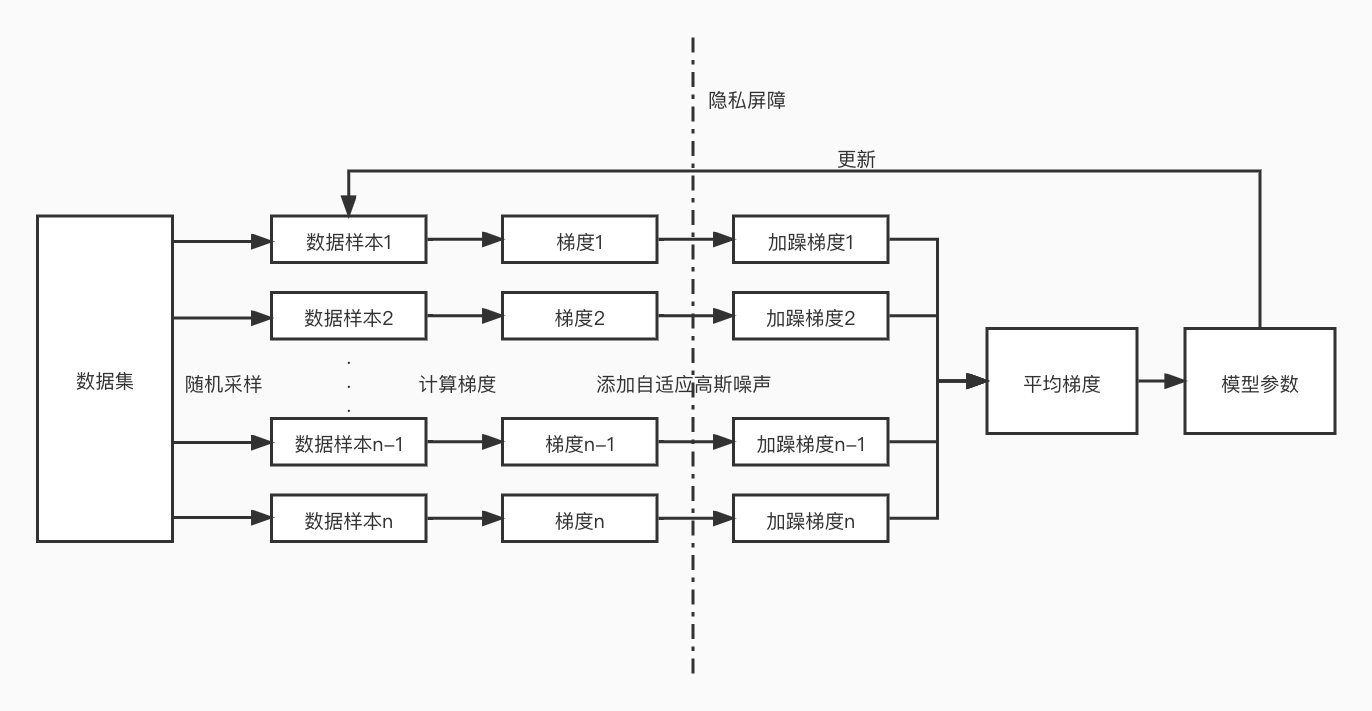
\includegraphics[scale=0.3]{fig2/C3/自适应差分隐私流程图}%联邦学习的系统架构
	\caption{自适应差分隐私流程图}
	\label{fig:自适应差分隐私流程图}	
\end{figure}

算法\ref{基于自适应差分隐私的随机梯度下降算法}详细描述了在本地客户端训练过程中,在随机梯度下降算法中添加自适应噪声使算法整体满足$(\epsilon, \delta)$-差分隐私,最小化目标函数$f(\theta)=\frac{1}{N} \sum_{k=1}^{N} f_{k}(\theta)$,并使用差分隐私组合定理分析整体的隐私预算。在随机梯度下降算法中,每一轮用户随机采样小批次的$B$个样本,对于样本集中的每条数据记录计算其梯度和其归因分数,根据梯度更新的方差和偏差选择合适$a_{t}$和$b_{t}$裁剪梯度。完成梯度裁剪后,对梯度添加同归因分数等比例的高斯噪声。之后计算批次大小$B$的样本集的平均加躁梯度,然后进行梯度下降,计算得到梯度更新的均值和标准差。之后不断重复采样迭代的进行梯度下降的训练,使目标函数最小,输出模型权重$\theta_{t}$。图\ref{fig:自适应差分隐私流程图}完整展示了本地设备进行模型训练的整个过程。

\begin{algorithm}[!htb]
	\caption{基于自适应差分隐私的随机梯度下降算法}
	\label{基于自适应差分隐私的随机梯度下降算法}
	\begin{algorithmic}[1]
		\footnotesize
		\STATE \textbf{输入:} 目标函数$f(\theta)=\frac{1}{N} \sum_{k=1}^{N} f_{k}(\theta)$,学习率$\eta^{t}$,训练批次大小$B$, 高斯噪声参数$\sigma$ 
		\STATE 初始化:$m^{0}=0 \cdot 1, s^{0}=\sqrt{h_{1} h_{2}} \cdot 1$
		\STATE 随机初始化模型参数:$\theta^{0}$
		\FOR{ $t \in[T]$}
			\FOR{ $i=1$ to $d$}
				\STATE $b_{i}^{t}=\sqrt{s_{i}^{t}} \cdot \sqrt{\sum_{i=1}^{d} s_{i}^{t}}$
			\ENDFOR
			\STATE 随机采样:$S_{t} \leftarrow B$
			\FOR{$k \in S_{t}$}
				\STATE 计算梯度:$\mathbf{g}_{t}\left(x_{i}\right) \leftarrow \nabla_{\theta_{t}} \mathcal{L}\left(\theta_{t}, x_{i}\right)$
				\STATE 计算梯度的归因分数:$\beta=\frac{\left|\ddot{C}_{j}\right|}{\sum_{j=1}^{u}\left|\ddot{C}_{j}\right|}$
				\STATE 梯度变换:$w_{i}^{t}=\frac{g_{i}^{t}-a_{i}^{t}}{b_{i}^{t}}$
				\STATE 梯度裁剪: $\hat{w}^{t}=\operatorname{clip}\left(w^{t}, 1\right) \triangleq \frac{w^{t}}{\max \left(1,\left\|w^{t}\right\|_{2}\right)}$
				\STATE 梯度复原: $\tilde{g}^{t}=b^{t} \tilde{w}^{t}+a^{t}$
				\STATE 根据归因分数分配相应的隐私预算:$\sigma==\frac{u *\left|\ddot{C}_{j}\right|}{\sum_{j=1}^{u}\left|\ddot{C}_{j}\right|} * \sigma_{l}$
				\STATE 添加高斯噪声:$\tilde{\mathbf{g}}_{t} \leftarrow \frac{1}{L} \sum_{i}\left(\overline{\mathbf{g}}_{t}\left(x_{i}\right)+\frac{1}{\left|D_{i}^{t}\right|}\mathcal{N}\left(0, S_{f}^{2} \cdot \sigma^{2}\right)\right)$
			\ENDFOR
			\STATE 计算加躁后的平均梯度:$\tilde{g}^{t}=\frac{1}{B} \sum_{k \in S_{t}} \tilde{g}^{t}(k)$
			\STATE 梯度下降:$\theta^{t+1}=\theta^{t}-\eta^{t} \tilde{g}^{t}$
			\STATE 根据\ref{eq:梯度方差估计}和\ref{eq:梯度偏差估计}更新均值和标准差
		\ENDFOR
		\STATE \textbf{输出:} $\theta_{t}$和整体隐私预算$(\epsilon, \delta)$
	\end{algorithmic}
\end{algorithm}

在本章接下来的两节,我们将给出自适应差分隐私随机优化算法关于隐私保证和模型效用性的证明,并与前人的方案进行对比。

\section{隐私性和收敛性证明}

\subsection{隐私性证明}
自适应差分SGD算法在梯度下降过程中根据梯度的归因分数在梯度上添加高斯噪声,算法整体满足$\left(\epsilon_{c}+\epsilon_{l}\right)$差分隐私。证明如下:

假设现有相邻数据集$D$和$D^{\prime}$,两个数据集上的数据记录$x_{n}$和$x_{n}^{\prime}$不同,$C(D)$和$C(D^{\prime})$分别代表这两个数据集上所有属性值的归因分数之和:

\begin{equation}
C(D)=\left\{C_{j}\left(x_{i}\right)\right\}, j \in[1, u], \text {其中} C_{j}\left(x_{i}\right)=\frac{1}{n} \sum_{i=1}^{n} C_{x_{i, j}}\left(x_{i}\right), j \in[1, u], x_{i} \in D
\end{equation}

\begin{equation}
C\left(D^{\prime}\right)=\left\{C_{j}\left(x_{i}^{\prime}\right)\right\}, j \in[1, u], \text {其中} C_{j}\left(x_{i}^{\prime}\right)=\frac{1}{n} \sum_{i=1}^{n} C_{x_{i, j}^{\prime}}\left(x_{i}^{\prime}\right), j \in[1, u], x_{i}^{\prime} \in D^{\prime}
\end{equation}

根据梯度的归因分数添加自适应的噪声,其中隐私预算与归因分数成正比:$\sigma$=$\sigma_{j}=\frac{u *\left|\ddot{C}_{j}\right|}{\sum_{j=1}^{u}\left|\ddot{C}_{j}\right|} * \sigma_{l}$:
\begin{equation}\label{eq:神经网络加噪3}
x_{i, j}^{\prime}=x_{i, j}+\frac{1}{\left|D_{i}^{t}\right|}\mathcal{N}\left(0, S_{f}^{2} \cdot \sigma^{2}\right)
\end{equation}

通过敏感度公式计算梯度归因分数的全局敏感度$GS_{c}$:
\begin{equation}\label{eq:贡献敏感度}
\begin{aligned}
G S_{c} &=\frac{1}{|D|} \sum_{j=1}^{u}\left\|\sum_{x_{i} \in D} C_{x_{i, j}}\left(x_{i}\right)-\sum_{x_{i}^{\prime} \in D^{\prime}} C_{x_{i, j}^{\prime}}\left(x_{i}^{\prime}\right)\right\|_{1} \\
&=\frac{1}{|D|} \sum_{j=1}^{u}\left\|C_{x_{n, j}}\left(x_{n}\right)-C_{x_{n, j}^{\prime}}\left(x_{n}^{\prime}\right)\right\|_{1} \\
& \leq \frac{2}{|D|} \max \sum_{j=1}^{u}\left\|C_{x_{i, j}}\left(x_{i}\right)\right\|_{1} \\
& \leq \frac{2 u}{|D|}
\end{aligned}
\end{equation}

其中,$u$和$|D|$分别表示属性和元组的数量,然后可以得到:
\begin{equation}\label{贡献数量和元组}
\begin{aligned}
\frac{\operatorname{Pr}(\ddot{C}(D))}{\operatorname{Pr}\left(\ddot{C}\left(D^{\prime}\right)\right)} &=\frac{\prod_{j=1}^{u} \exp \left(\frac{\epsilon_{c}\left\|\frac{1}{|D|} \sum_{x_{i} \in D} C_{j}\left(x_{i}\right)-\ddot{C}_{j}\left(x_{i}\right)\right\|_{1}}{G S_{c}}\right)}{\prod_{j=1}^{u} \exp \left(\frac{\epsilon_{c}\left\|\frac{1}{\left|D^{\prime}\right|} \sum_{x_{i}^{\prime} \in D^{\prime}} C_{j}\left(x_{i}^{\prime}\right)-\ddot{C}_{j}\left(x_{i}^{\prime}\right)\right\|_{1}}{G S_{c}}\right)} \\
&=\prod_{j=1}^{u} \exp \left(\frac{\epsilon_{c}}{|D| G S_{c}}\left\|C_{j}\left(x_{n}\right)-C_{j}\left(x_{n}^{\prime}\right)\right\|_{1}\right) \\
& \leq \prod_{j=1}^{u} \exp \left(\frac{\epsilon_{c}}{|D| G S_{c}} \max \left\|C_{j}\left(x_{n}\right)\right\|_{1}\right) \\
&=\exp \left(\epsilon_{c} \frac{\max _{x_{i} \in D} \sum_{j=1}^{u}\left\|C_{j}\left(x_{n}\right)\right\|_{1}}{|D| G S_{c}}\right) \\
& \leq \exp \left(\epsilon_{c}\right)
\end{aligned}
\end{equation}

因此,根据梯度归因分数添加高斯噪声的算法是满足$\epsilon_{c}$-差分隐私的。
接着我们根据归因分数对于梯度进行概率选择添加噪声,我们接下来证明这部分的算法是满足$\epsilon_{l}$-差分隐私的。

假设两个相邻的数据集$D_{i}^{t}$和$D_{i}^{t^{\prime}}$,其中数据记录$x_{n}$和$x_{n}^{\prime}$不同,$z\left(D_{i}^{t}\right)$和$z\left(D_{i}^{t^{\prime}}\right)$分别为两个数据集上训练采用的线性变换函数。

一般来说,我们把偏置项视为第一类数据属性,即:$x_{i,0}=b_{i}$。线性转换可以改写为:$\ddot{\mathbf{z}}_{x \in D_{i}^{t}}(\omega)=\ddot{\mathbf{x}} * \omega$。线性变换函数的敏感度$G S_{l}$为:
\begin{equation}
\begin{aligned}
G S_{l} &=\sum_{a_{i} \in l_{1}} \sum_{j=1}^{u}\left\|\sum_{x_{i} \in D_{i}^{t}} x_{i, j}-\sum_{x_{i}^{\prime} \in D_{i}^{t^{\prime}}} x_{i, j}^{\prime}\right\|_{1} \\
&=\sum_{a_{i} \in l_{1}} \sum_{j=1}^{u}\left\|x_{n, j}-x_{n, j}^{\prime}\right\|_{1} \\
& \leq \sum_{a_{i} \in l_{1}} \sum_{j=1}^{u} \max _{x_{i} \in D_{i}^{t}}\left\|x_{n, j}\right\|_{1} \\
& \leq \sum_{a_{i} \in l_{1}} u
\end{aligned}
\end{equation}

其中,$a_{i} \in l_{1}$是指第一个隐藏层$l_{1}$中的神经元$a_{i}$,$u$是数据元组$x_{i} \in D_{i}^{t}$中的属性数。自适应加躁算法包括两个超参数:$f$和$p$,这两个超参数可以适时过滤多余的噪声,再通过超参数调整噪声大小和裁剪阈值后,整体加躁后的梯度的表达式如下:
\begin{equation}
\begin{aligned}
\tilde{x}_{i, j} &=[(1-f)+f * p] * \ddot{x}_{i, j}+f *(1-p) * x_{i, j} \\
&=[(1-f)+f * p]\left[x_{i, j}+\mathcal{N}\left(0, S_{f}^{2} \cdot \sigma^{2}\right)\right]+[f *(1-p)] x_{i, j} \\
&=x_{i, j}+[(1-f)+f * p]\left[\mathcal{N}\left(0, S_{f}^{2} \cdot \sigma^{2}\right)\right]
\end{aligned}
\end{equation}
然后我们可以得到:

\begin{equation}
\begin{aligned}
\frac{\operatorname{Pr}\left(\ddot{\mathbf{z}}_{D_{i}^{t}}(\omega)\right)}{\operatorname{Pr}\left(\ddot{\mathbf{z}}_{D_{i}^{t}}(\omega)\right)} &=\frac{\prod_{a_{i} \in l_{1}} \prod_{j=1}^{u} \exp \left(\frac{\epsilon_{j}\left\|\sum_{x_{i} \in D_{i}^{t}} x_{i, j}-\sum_{x_{i} \in D_{i}^{t}} \tilde{x}_{i, j}\right\|_{1}}{G S_{l}}\right)}{\prod_{a_{i} \in l_{1}} \prod_{j=1}^{u} \exp \left(\frac{\epsilon_{j}\left\|\sum_{x_{i}^{\prime} \in D_{i}^{t^{\prime}}} x_{i, j}^{\prime}-\sum_{x_{i}^{\prime} \in D_{i}^{t^{\prime}}} \tilde{x}_{i, j}^{\prime}\right\|_{1}}{G S_{l}}\right)} \\
& \leq \prod_{a_{i} \in l_{1}} \prod_{j=0}^{u} \exp \left(\frac{\epsilon_{j}}{G S_{l}}\left\|\sum_{x_{i} \in D_{i}^{t}} x_{i, j}-\sum_{x_{i}^{\prime} \in D_{i}^{t^{\prime}}} x_{i, j}^{\prime}\right\|_{1}\right) \\
& \leq \prod_{a_{i} \in l_{1}} \prod_{j=0}^{u} \exp \left(\frac{\epsilon_{j}}{G S_{l}} \max _{x_{i} \in D_{i}^{t}}\left\|x_{n, j}\right\|_{1}\right) \\
& \leq \exp \left(\epsilon_{l} \frac{\sum_{a_{i} \in l_{1}} u\left[\sum_{j=1}^{u} \frac{\left|\ddot{C}_{j}\right|}{\sum_{j=1}^{u}\left|\ddot{C}_{j}\right|}\right]}{G S_{l}}\right) \\
&=\exp \left(\epsilon_{l}\right)
\end{aligned}
\end{equation}

根据上述推倒证明可知,在联邦学习的神经网络中添加自适应噪声后,所上传的梯度是满足$\left(\epsilon_{c}+\epsilon_{l}\right)$-差分隐私的。在满足差分隐私的基础上,在下一节我们结合差分隐私的组合定理,计算累积的隐私预算。

\subsection{隐私参数分析}
本章所提出的自适应差分隐私保护方案是通过在随机梯度下降算法上添加自适应的高斯噪声,保护数据的隐私性。在上一节我们已经证明了此算法满足$\left(\epsilon_{c}+\epsilon_{l}\right)$差分隐私,那另外一个非常重要的问题就是评估在训练过程中添加噪声所累积的隐私预算成本。

我们向梯度中添加高斯噪声以得到加躁后的数据,根据第二章所给出的高斯机制的定理可知,当隐私参数$\sigma=\sqrt{2 \log \frac{1.25}{\delta}} / \varepsilon$时,每一批次的输出都满足$(\varepsilon, \delta)$-差分隐私。考虑到训练批次是以概率$q=L / N$从数据集中随机采样的,根据隐私放大定理和差分隐私的强组合定理,隐私性由$(\varepsilon, \delta)$-差分隐私扩大到 $(q \varepsilon, q \delta)$-差分隐私。

然而,组合定理并没有考虑到特定的噪声分布,给出的隐私边界较为松散。在本节中,我们采用“Moments Accountant”(MA)机制,去计算算法迭代过程中添加噪声所累积的隐私预算成本。MA机制通过跟踪隐私损失随机变量随时间的变化,并结合组合定理,对于采样的高斯机制给出更严格的隐私损失估计。

隐私损失是一个随机变量,取决于添加到算法中的随机噪声。假使算法$\mathcal{M}$是满足 $(\varepsilon, \delta)$-差分隐私的,那么$\mathcal{M}$中的隐私损失随机变量是存在严格的尾部边界。尾部边界在概率分布中是一个非常重要的信息。我们通过计算隐私损失随机变量的对数矩
,结合标准的马尔科夫不等式,得到尾部边界,也差分隐私算法的隐私损失。

对于邻近数据集 $d, d^{\prime} \in \mathcal{D}^{n}$,算法$\mathcal{M}$,额外输入aux,算法的输出$o \in \mathcal{R}$的隐私损失表示为:
$$
c\left(o ; \mathcal{M}, \mathrm{aux}, d, d^{\prime}\right) \triangleq \log \frac{\operatorname{Pr}[\mathcal{M}(\mathrm{aux}, d)=o]}{\operatorname{Pr}\left[\mathcal{M}\left(\mathrm{aux}, d^{\prime}\right)=o\right]}
$$

由于在随机梯度下降算法$\mathcal{M}$中,通过迭代的梯度下降更新权重,每一轮输出的梯度满足差分隐私,根据差分隐私的串行组合定理,最终的模型输出也满足差分隐私。我们定义第$\lambda^{\text {th }}$个时刻的时刻生成函数:
$$
\begin{aligned}
\alpha_{\mathcal{M}}(\lambda ; \operatorname{aux},&\left.d, d^{\prime}\right) \triangleq\log \mathbb{E}_{o \sim \mathcal{M}(\operatorname{aux}, d)}\left[\exp \left(\lambda c\left(o ; \mathcal{M}, \text { aux }, d, d^{\prime}\right)\right)\right]
\end{aligned}
$$

为了证明给定算法$\mathcal{M}$的隐私保障,我们对于每一轮的$\alpha_{\mathcal{M}}\left(\lambda ;\right.$ aux $\left., d, d^{\prime}\right)$给出严格的尾部边界,考虑到所有可能的额外输入和邻近数据集$\left., d, d^{\prime}\right)$,整体的时刻函数为:
$$
\alpha_{\mathcal{M}}(\lambda) \triangleq \max _{\text {aux }, d, d^{\prime}} \alpha_{\mathcal{M}}\left(\lambda ; \text { aux }, d, d^{\prime}\right)
$$

$\alpha_{\mathcal{M}}(\lambda)$满足串行组合定理和尾部边界定理:

\begin{theorem}[时刻函数的串行组合]\label{时刻函数的串行组合}
假设算法$\mathcal{M}$是由一系列自适应算法$\mathcal{M}_{1}, \ldots, \mathcal{M}_{k}$组合而成的,满足$\mathcal{M}_{i}: \prod_{j=1}^{i-1} \mathcal{R}_{j} \times \mathcal{D} \rightarrow \mathcal{R}_{i}$,那么对于任意的$\lambda$都满足:
$$
\alpha_{\mathcal{M}}(\lambda) \leq \sum_{i=1}^{k} \alpha_{\mathcal{M}_{i}}(\lambda)
$$
\end{theorem}

\begin{theorem}[时刻函数的尾部边界]\label{时刻函数的尾部边界}
对于任意的 $\varepsilon>0$,算法$\mathcal{M}$是满足$(\varepsilon, \delta)$-差分隐私的,当
$$
\delta=\min _{\lambda} \exp \left(\alpha_{\mathcal{M}}(\lambda)-\lambda \varepsilon\right)
$$
\end{theorem}

根据定理\ref{时刻函数的尾部边界},在算法的每一次迭代中,通过计算$\alpha_{\mathcal{M}_{i}}(\lambda)$然后限定其尾部边界,结合\ref{时刻函数的串行组合},就可以得到整体时刻函数的尾部边界,通过隐私损失变量的尾部边界计算得到整体的隐私损失。


\section{实验评估}
\subsection{实验准备}
在这一节中,我们进行实验来评估本地自适应差分隐私在联邦学习系统中的性能。在模拟的联邦学习系统中,我们假设有四台本地设备,每个本地用户由配备6GB内存、四核2.36GHz Cortex A73处理器和四核Cortex A53 1.8GHz处理器的华为nova3安卓手机模拟。中央服务器由两台联想服务器模拟的,这两台服务器有2个英特尔(R)至强(R)E5-2620 2.10GHZ CPU,32GB内存,512SSD,2TB机械硬盘,运行于Ubuntu 18.04操作系统。

在实验过程中,我们选择了深度学习中常用的两个经典数据集--MNIST手写体数字识别数据集\upcite{ref46}和CIFAR-10数据集\upcite{ref68}进行实验。
\begin{itemize}
\item MNIST数据集包含60000个训练样本和10000个测试样本。MNIST是用于分类任务的经典数据集,来源于美国国家标准与技术研究所。总共包含60000个训练样本和10000个测试样本。每个样本为28x28像素的手写数字图像,每个像素点用灰度值表示,灰度值范围为0到255,图像包含十个类别,如下图\ref{fig:MNIST手写数字数据集}所示。

\item CIFAR-10数据集包含了十个类别的RGB彩色图像,总共包含50000个训练样本和10,000个测试岩本。每张图像的大小为32*32。这些图像有以下十个类别:飞机、汽车、鸟、猫、鹿、狗、青蛙。马,船,和卡车。

\end{itemize}


\begin{figure}[!hbt]
\centering
	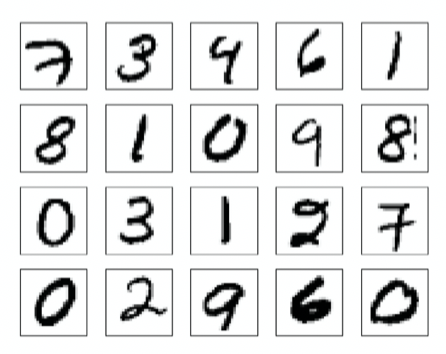
\includegraphics[scale=0.6]{fig2/C3/MNIST}%联邦学习的系统架构
	\caption{MNIST手写数字数据集}
	\label{fig:MNIST手写数字数据集}	
\end{figure}

此外,我们让所有用户离线训练一个统一的卷积神经网络,以获得本地用户的梯度。在我们的实验中采用的模型网络结构为CNN,包括2个卷积层(分别包含20个特征图和50个特征图),两个池化层层和两个全连接层(分别为256和10个神经元)。模型的激活函数为ReLU,并引入了DropOut正则以提高模型的泛化能力。图\ref{fig:CNN模型网络结构}展示了CNN的网络结构。

\begin{figure}[!hbt]
\centering
	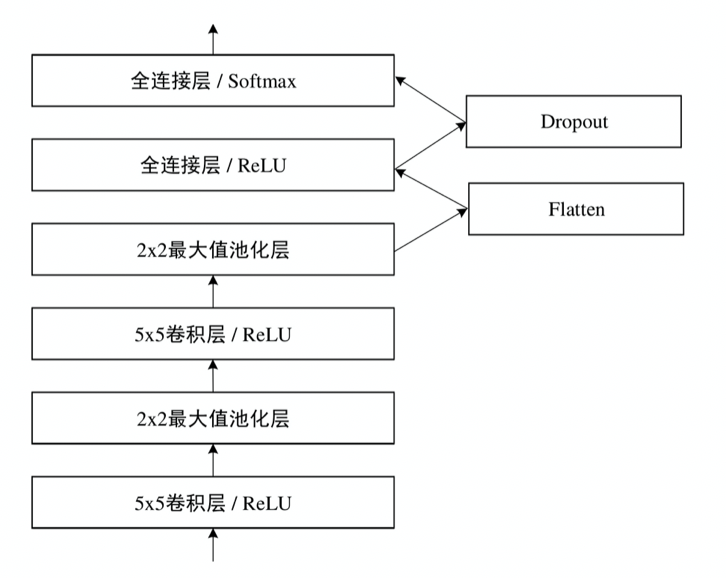
\includegraphics[scale=0.6]{fig2/C3/CNN网络结构}%联邦学习的系统架构
	\caption{模型网络结构}
	\label{fig:CNN模型网络结构}	
\end{figure}

所有的实验都是用PYTHON语言编译的,我们使用Tensorflow去实现本地差分隐私算法,这是一个流行的深度学习库。 本文使用了TensorFlow-Federated,这是TensorFlow中的一个联合学习库。我们在Python的基础上二次开发了该算法,并通过将该算法部署到多个边缘设备上构建了一个真实的联合学习环境。以本地训练集MNIST为例,图\ref{fig:仿真联邦系统模型概览}展示了联邦学习的仿真模型概览。

\begin{figure}[!hbt]
\centering
	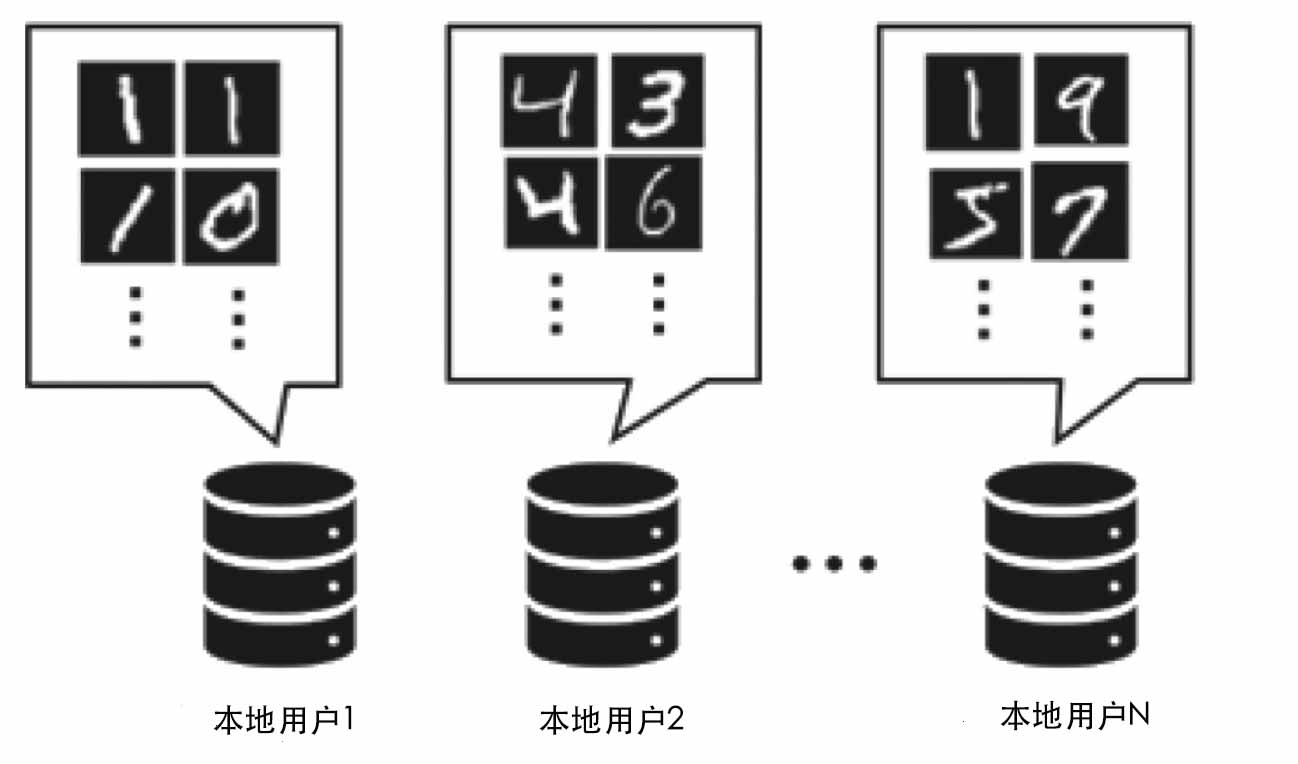
\includegraphics[scale=0.6]{fig2/C3/联邦系统仿真模型概览}%联邦学习的系统架构
	\caption{仿真联邦系统模型概览}
	\label{fig:仿真联邦系统模型概览}	
\end{figure}

\subsection{实验设计}
为了实现隐私保护,我们需要在本地训练的随机梯度下降算法中实现梯度的自适应扰动,并采用MA机制跟踪每一次梯度扰动所增加的隐私预算。因此,代码的实现主要分为两个部分:梯度扰动(Sanitizer),隐私预算跟踪(Accountant)。

图\ref{fig:实现本地自适应差分隐私的伪代码片段}展示了实现梯度扰动和隐私预算跟踪的代码片段,为了实现整体算法满足$\left(\epsilon_{c}+\epsilon_{l}\right)$-差分隐私,Sanitizer需要完成以下三个步骤:首先,通过前向传播算法计算每批样本的梯度及其归因分数;其次,根据每个样本的梯度范数进行梯度裁剪以限制函数敏感度;最后,根据归因分数在梯度上添加自适应的噪声然后更新权重。

\begin{figure}[!hbt]
\centering
	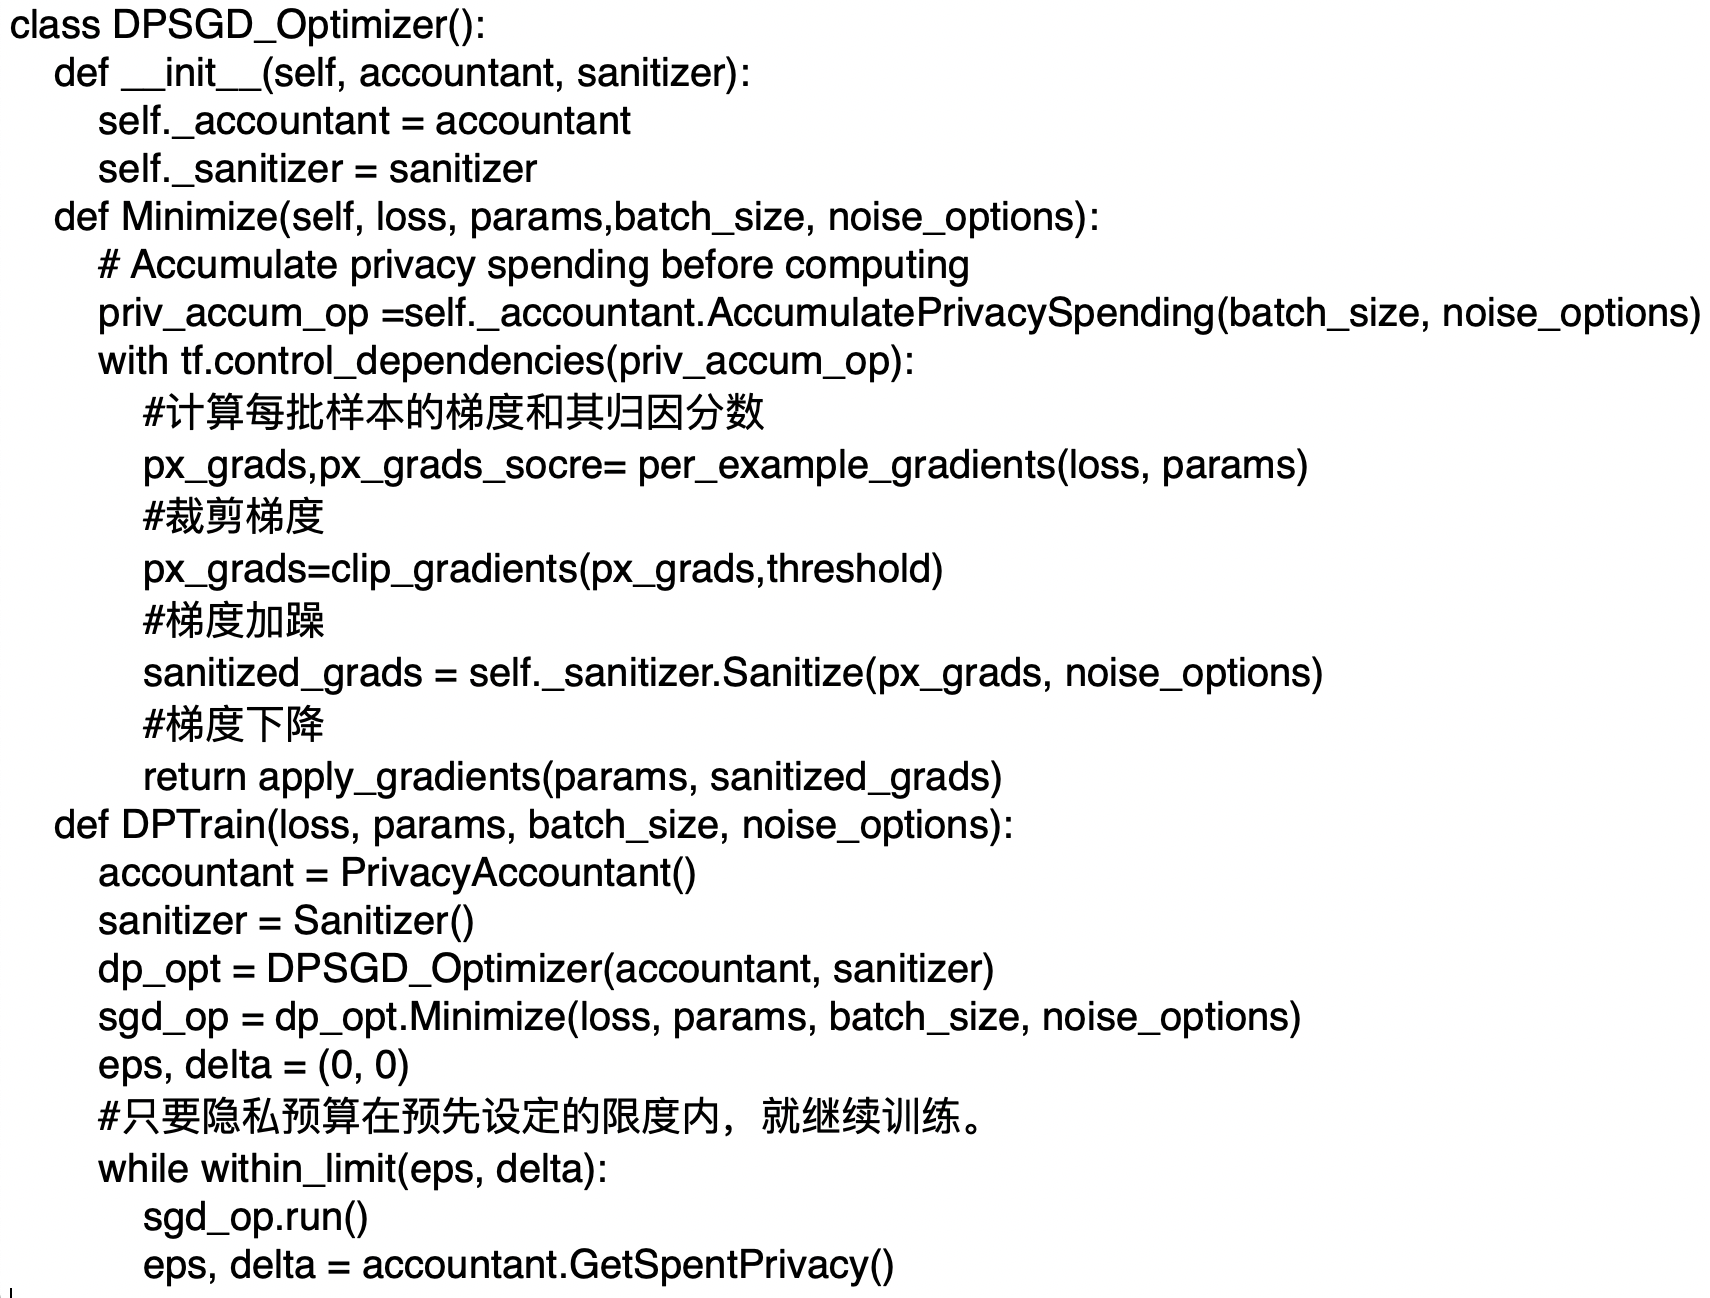
\includegraphics[scale=0.5]{fig2/C3/代码片段1}%联邦学习的系统架构
	\caption{实现本地自适应差分隐私的伪代码片段}
	\label{fig:实现本地自适应差分隐私的伪代码片段}	
\end{figure}

在TensorFlow中,由于性能原因,梯度计算是分批进行的,所以在训练过程,随机采样一批训练子样本$B$:
$\mathbf{g}_{B}=1 /|B| \sum_{x \in B} \nabla_{\theta} \mathcal{L}(\theta, x)$
。为了限制梯度更新的敏感度,我们需要计算每个批次的梯度$\nabla_{\theta} \mathcal{L}(\theta, x)$,具体由per\_example\_gradients函数实现。这样即使是大批量的训练,训练速度也不会大幅下降。在每个批次的训练中,我们会单独计算损失函数 
$\mathcal{L}$,也就是每个数据样本$x_{i}$都有单独的损失函数结果$\mathcal{L}$。一旦我们获得了每批数据样本的梯度,
我们可以很容易地使用TensorFlow操作符来对梯度进行裁剪,添加噪音。

我们的实验主要分为三个部分:
\begin{enumerate}
\item [(1)] 针对本地自适应差分隐私方案,分析噪声水平、裁剪阈值、隐藏层数量这些超参数对模型分类准确率影响。
\item [(2)] 将本地自适应差分隐私方案与基准方案、前人提出的差分隐私SGD方案(如表所示)进行对比,评估指标为模型分类准确率和隐私预算。
\item [(3)] 在本地自适应差分隐私的联邦学习模型上应用成员推理进行攻击实验,评估模型的隐私保护效用。

\begin{table}[H]
	\centering
	\begin{tabular}{cc}
		\hline
		基准方案名称& 具体算法\\
		\hline
		SGD& 没有实现差分隐私的随机梯度下降算法\\
		DP-SGD\upcite{ref57}& 在梯度上添加固定噪声大小的差分隐私随机梯度下降算法\\
		DS-SGD\upcite{ref67}& 在梯度下降过程中,选择性的进行参数共享实现隐私保护\\
		LDP-SGD& 本地差分隐私方案\\
		\hline
	\end{tabular}
	\caption{本地自适应差分隐私与其他四种基准方案}
	\label{tab1}
\end{table}

\end{enumerate}

\subsection{结果分析}

\subsubsection{实验一(分析各个参数对模型准确率的影响)} 
分类模型的精度由多个因素决定,必须仔细调整以获得最佳性能。这些因素包括网络的拓扑结构、隐藏单元的数量以及训练程序的参数,如批量大小和学习率。有些参数是针对隐私的,如梯度规范剪裁边界和噪声水平。本节实验重点研究噪声大小,裁剪阈值和隐藏层数量这三个参数对于模型分类准确率的影响。为了准确的反映每种参数对于准确率的影响,我们控制其余变量。参考值如下:1,000个隐性单元,600个批量,梯度范数边界为4,初始学习率为0.1,在10个训练轮次中递减到最终学习率为0.052,噪声参数$\sigma$分别为0.2和0.5,用于训练CNN网络模型。对于每一种参数组合进行模型训练,直至隐私预算累积至$\left(2,10^{-5}\right)$-差分隐私。具体的实验结果如图\ref{fig:在MNIST数据集上噪声大小,裁剪阈值和隐藏层数量这三个参数对于训练准确率的影响}所示。

\begin{figure}[!hbt]
\centering
	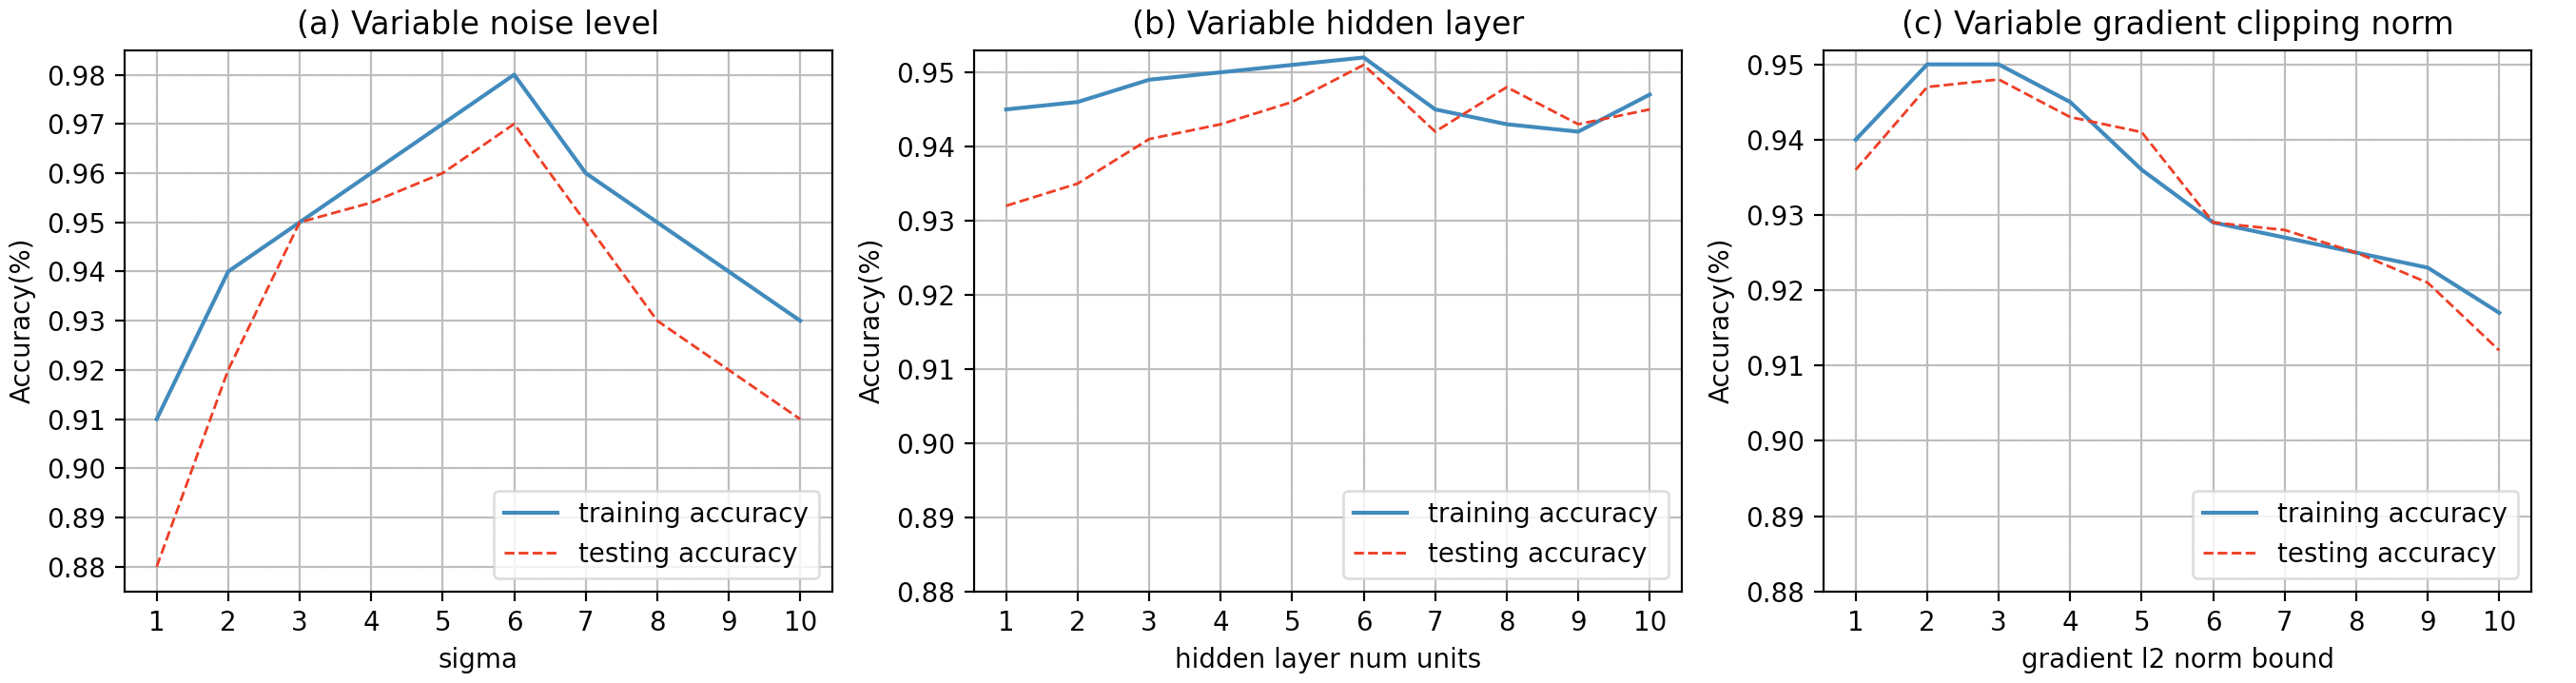
\includegraphics[scale=0.32]{fig2/C3/第三章实验一}%联邦学习的系统架构
	\caption{在MNIST数据集上噪声大小,裁剪阈值和隐藏层数量这三个参数对于训练准确率的影响}
	\label{fig:在MNIST数据集上噪声大小,裁剪阈值和隐藏层数量这三个参数对于训练准确率的影响}	
\end{figure}

如图\ref{fig:在MNIST数据集上噪声大小,裁剪阈值和隐藏层数量这三个参数对于训练准确率的影响}(a)展示的是噪声参数$\sigma$对模型准确率的影响,X轴是噪声水平,这个值的选择对准确性有很大影响。通过添加更多的噪音,每步的隐私损失成比例缩小,所以我们可以在给定的累积隐私预算内运行更多的训练轮次。准确率维持在0.88\%至0.98\%之间,我们的框架允许对训练参数进行自适应控制减少了过拟合情况,自适应的噪声添加同时提高了模型的准确性和训练性能。

图\ref{fig:在MNIST数据集上噪声大小,裁剪阈值和隐藏层数量这三个参数对于训练准确率的影响}(b)展示了隐藏层数量对模型准确率的影响,X轴表示隐藏层单元数量。对于非差分隐私模型,更多的隐藏单元能有效避免过度拟合,因为更多的隐藏单元会让我们的训练更有针对性。然而,添加了差分隐私的模型训练,隐藏层数量的增加可能会影响梯度的敏感度,使每次梯度更新时添加更多的噪声。然而我们的根据梯度的归因分数自适应添加噪声的方案能有效的控制敏感度有界,随着隐藏单位的数量增加,模型的准确率依然维持在93\%以上。

图\ref{fig:在MNIST数据集上噪声大小,裁剪阈值和隐藏层数量这三个参数对于训练准确率的影响}(c)展示了梯度范数阈值对模型准确率的影响,X轴表示梯度$l2$范数阈值C。当C为2-3时,模型准确率最高,接着随着C的增加,模型准确率逐渐降低至91\%左右,限制梯度范数会产生两个相反的效果:剪裁破坏了梯度估计的无偏性,如果剪裁参数太小,被剪切的平均梯度可能与真实梯度的方向大不相同。另一方面,增加梯度范数迫使我们在梯度中加入更多的噪声,也就是以σC的比例添加噪声。而我们的自适应梯度裁剪方案能有效的考虑上一轮训练得到的梯度偏差和方差,取训练过程中未被剪辑的梯度范数的中值,模型准确率最高依然能达到95\%左右。

对于不同隐私预算的训练版本,我们用同样的架构进行了实验:一个包括1000个神经元的ReLU隐藏层,以及600个批量大小。为了限制敏感度,我们设置每个神经层的梯度范数阈值为4。我们报告了四种噪声规模的训练结果,分别为小(σ=2)、中(σ=4)、大(σ=8)和更大(10)。这里σ代表训练神经网络的噪声水平。学习率最初设置为0.1,在10个历时中线性下降到0.052,然后固定为0.052。

图\ref{fig:在MNIST数据集上不同噪声水平下训练的准确率}显示了不同噪音水平下的训练的结果,在每张图中,我们都显示了训练和测试准确率的变化情况。对于噪声参数为$\left(2,10^{-5}\right)$,$\left(4,10^{-5}\right)$,$\left(8,10^{-5}\right)$和$\left(10,10^{-5}\right)$的差分隐私,分别达到92\%、94\%、95\%和97\%的测试集准确性。我们的自适应差分隐私SGD方案,使模型在训练集和测试集上的准确度差异很小,这与理论上的观点一致,即添加噪声后的梯度训练依然有很好的泛化作用。相比之下,非差分隐私SGD的训练和测试准确率之间的差距随着训练轮次的增加而增加,容易造成过拟合。在噪声参数为$\left(10,10^{-5}\right)$时,模型在200个训练轮次后能达到接近非差分隐私模型的准确率。

\begin{figure}[!hbt]
\centering
	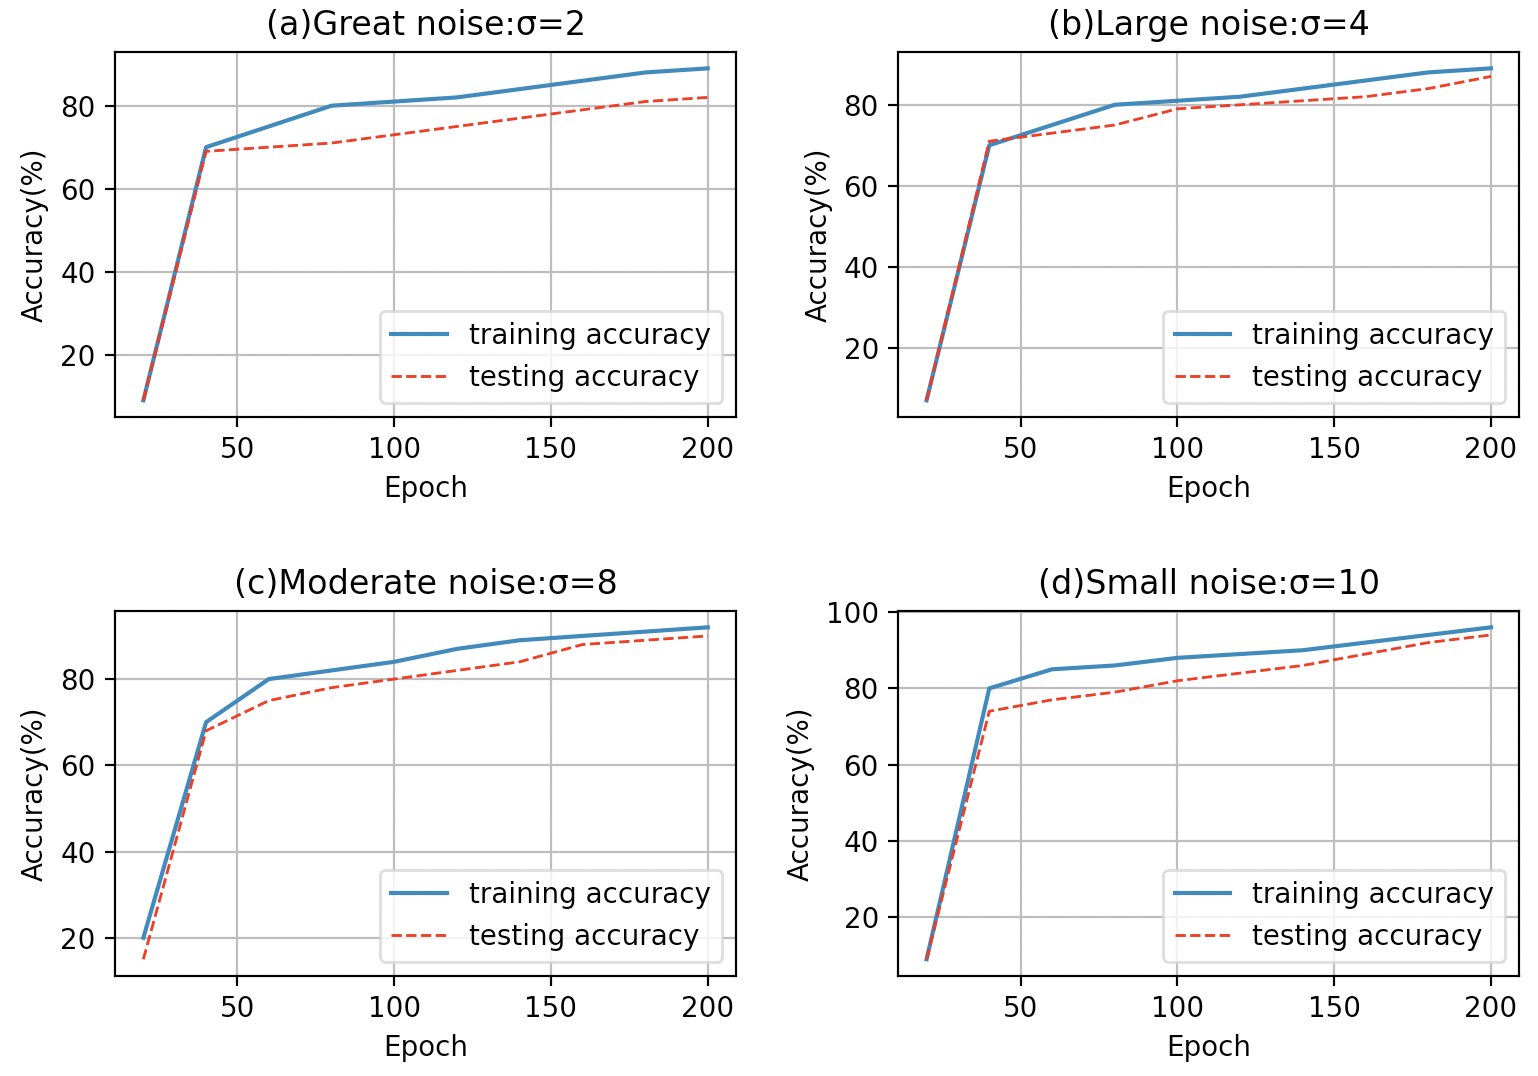
\includegraphics[scale=0.35]{fig2/C3/第三章实验一2}%联邦学习的系统架构
	\caption{在MNIST数据集上不同噪声水平下训练的准确率}
	\label{fig:在MNIST数据集上不同噪声水平下训练的准确率}	
\end{figure}

\subsubsection{实验二(与前人的隐私保护方案进行对比实验)} 
我们将本文提出的本地自适应差分隐私方案与SGD、DP-SGD、DS-SGD、LDP-SGD方案进行对比实验,选取的数据集为MNIST和CIFAR-10,网络模型为CNN5,具体的参数设置如下表所示。我们比较了不同方案在各个训练时长和迭代周期在测试集上所计算的目标函数的平均损失误差与梯度范数。

\begin{table}[H]
	\centering
	\begin{tabular}{ccc}
		\hline
		参数& MNIST& CIFAR-10\\
		\hline
		$\sigma$& 0.2/0.5& 0.2/0.5\\
		$k$& 0.7& 0.7\\
		梯度范数阈值& 20& 20\\
		学习率& 0.05& 0.05\\
		本地设备数量& 1000& 100\\
		训练轮数& 10& 10\\
		\hline
	\end{tabular}
	\caption{对比实验在数据集MNIST和CIFAR-10上的参数设置}
	\label{tab1}
\end{table}

图\ref{fig:不同隐私保护方案在MNIST(左列)和CIFAR-10(右列)数据集上训练的测试误差和梯度范数下降情况}显示了在隐私预算$\sigma$=0.2和$\sigma$=0.5的情况下,不同方案在MNIST数据集上随训练轮次平均测试误差和梯度范数变化情况的对比。

首先,对于MNIST数据集,在没有添加差分隐私保护的原始模型上进行梯度下降训练,经过20个训练轮次后模型在训练集上得到的基准准确率为99\%,我们的方案(Adaptive Differential Privacy-SGD,ADP-SGD)在训练刚开始的一个轮次,训练集的训练误差下降较慢,这是由于刚开始训练时模型中所有梯度的归因分数较高,导致对于每个梯度分配的隐私预算较高,加躁后与原始值差异较大。然而,在2个轮次过后,模型收敛的速度远远超过其他三个基准差分隐私方案。在5个训练轮次之后,训练集的损失率降低至25\%以下,而DS-SGD和DP-SGD的训练损失值在10个轮次之后仅降低至35\%左右,DP-SGD更次之,在40\%左右。相比于噪声参数$\sigma$=0.2,更大的噪声参数$\sigma$=0.5意味着更低的隐私预算,并且最终达到的模型精度也越高。图\ref{fig:不同隐私保护方案在MNIST(左列)和CIFAR-10(右列)数据集上训练的测试误差和梯度范数下降情况}中的(c1)和(d1)展示了模型训练中梯度的下降情况,在相同的隐私预算下,ADP-SGD能在2个训练轮次,梯度范数接近0.01且趋于平稳,意味着模型达到收敛的速度最快。

其次,对于CIFAR-10数据集,由于图像本身复杂度的增加,在没有添加差分隐私保护的原始模型上进行梯度下降训练,经过20个训练轮次后模型在训练集上得到的基准准确率为97\%。LDP在第一个训练轮次的模型收敛速率最高,然而在第二个训练轮次过后,ADP-SGD达到35\%的模型准确率和0.05左右的梯度范数,训练数据损失值和梯度范数均比另外三个基准方案的效果优。综上,我们的方案在调整梯度自适应加躁和自适应裁剪后使得模型收敛率和准确率大大提升。

\begin{figure}[!hbt]
\centering
	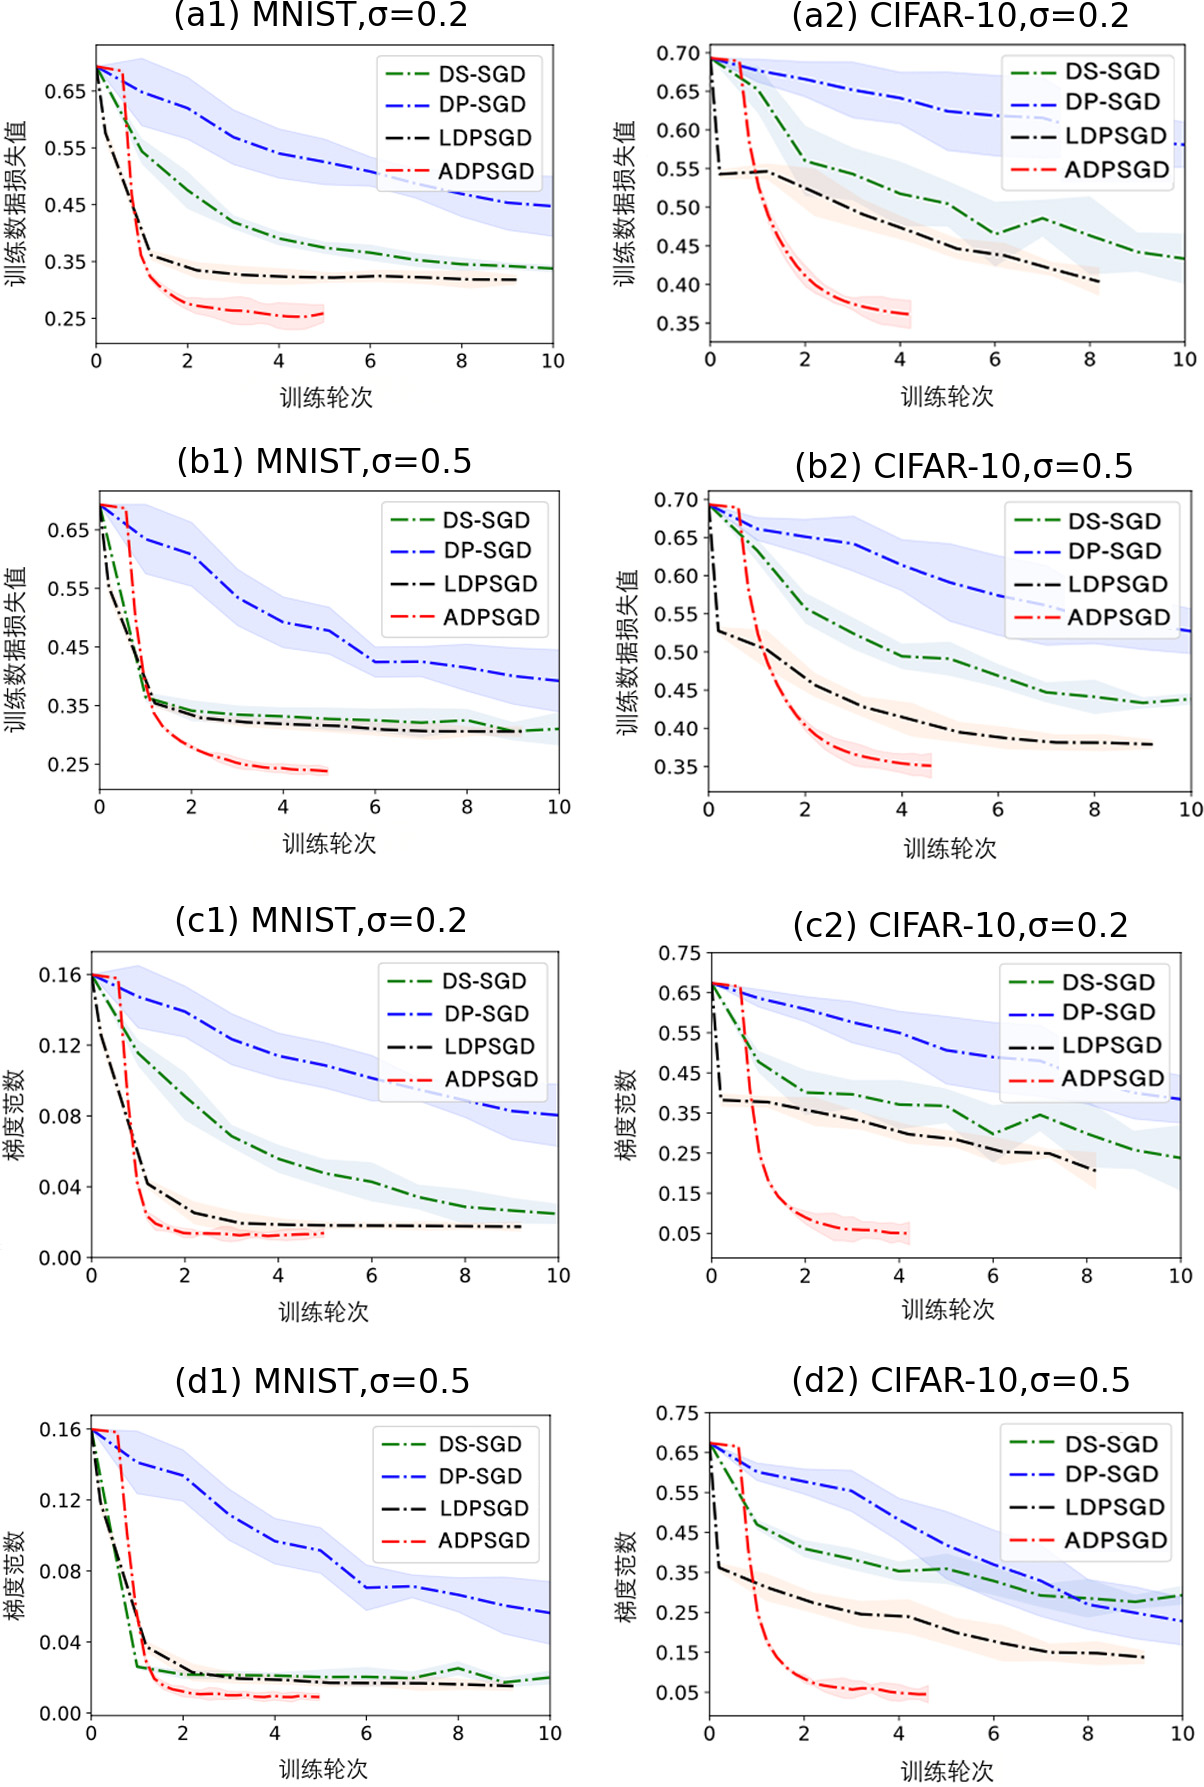
\includegraphics[scale=0.1]{fig2/C3/第三章实验二}%联邦学习的系统架构
	\caption{不同隐私保护方案在MNIST(左列)和CIFAR-10(右列)数据集上训练的测试误差和梯度范数下降情况}
	\label{fig:不同隐私保护方案在MNIST(左列)和CIFAR-10(右列)数据集上训练的测试误差和梯度范数下降情况}	
\end{figure}

\subsubsection{实验三(针对攻击模型,分析该方案的隐私保护效用)} 
我们曾在第一章介绍了针对联邦学习模型的隐私攻击,其中成员推理攻击是最流行的一类攻击,旨在确定一个输入样本x是否存在于模型训练集D中。该攻击只假设知道模型的输出预测向量(黑盒),并且是针对有监督的机器学习模型进行的。为了推断成员属性,对抗者使用与目标模型的相同算法训练了很多影子模型。对于每个影子模型,对手随机选择一些数据样本来形成一个训练集和一个评价集。影子模型是在训练集上训练的。然后,他将训练特征数据和验证特征数据都送入影子模型,并获得相应的结果,即每个类别的概率。所以对手可以建立一个分类器,以特征数据的预测结果为输入,以数据是来自训练集(表示为1)还是验证集(表示为0)为标签。有了这个分类器,对手将考虑中的敏感样本的特征值发送到目标模型并检索预测结果。然后,他将预测结果发送给分类器,并得到敏感样本是否是目标模型训练集的成员的结论。

我们重现了文献\upcite{ref70}中的成员推理攻击算法,配置和参数与之相同:目标模型是卷积神经网络,数据集为CIFAR-10。我们为目标模型和影子模型选择了两种规模的训练集:2500和10,000,验证集的大小与训练集相同。对手用不同的训练和验证样本子集运行100个影子模型。使用逻辑回归算法根据预测结果对样本是否包含在训练集中进行分类。

该实验的评估指标为模型的隐私保护效用,因此我们对比了针对自适应差分隐私和无隐私保护的模型进行成员推理攻击的攻击准确率,结果如图\ref{fig:在不同模型上进行成员推理攻击的准确率}所示。

\begin{figure}[!hbt]
\centering
	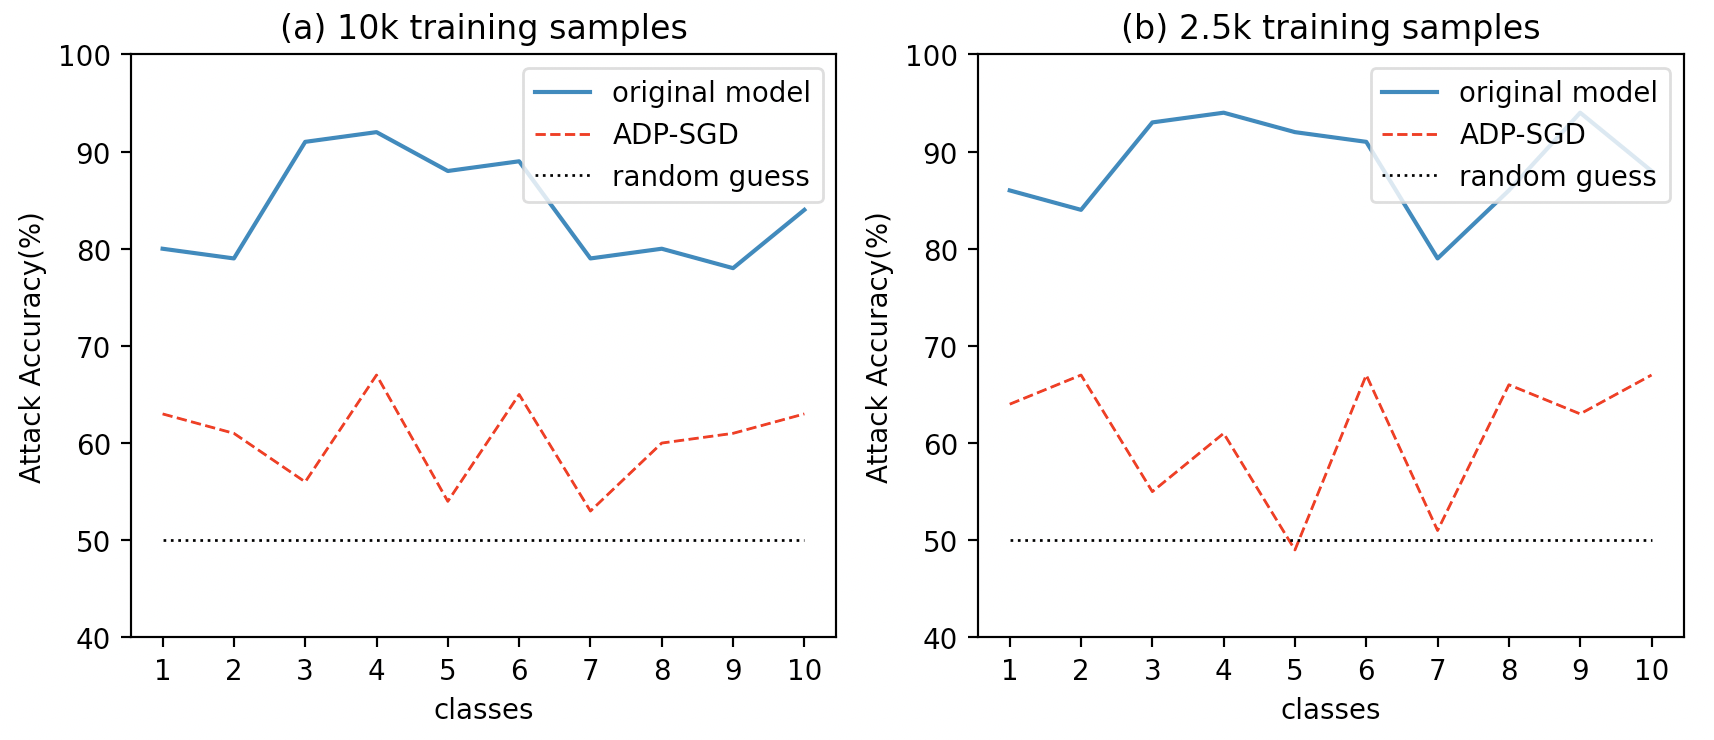
\includegraphics[scale=0.3]{fig2/C3/第三章实验三}%联邦学习的系统架构
	\caption{在不同模型上进行成员推理攻击的准确率}
	\label{fig:在不同模型上进行成员推理攻击的准确率}	
\end{figure}

我们分别在10k和2.5k个数据样本上进行攻击实验,图\ref{fig:在不同模型上进行成员推理攻击的准确率}中的(a)表示在10k数据样板上进行攻击实验,x轴表示对抗攻击的类别,蓝线(original model)表示在原始无隐私保护的模型上进行成员推理攻击的各个类别的攻击准确率,在不同类别上基本都可达到80\%~90\%的准确率。我们可以看到,对手对识别包含在训练集中的样本有很高的信心。当样本不在训练集中时,错误率相对较高。一般来说,F1分数非常高(0.86和0.89)。图\ref{fig:在不同模型上进行成员推理攻击的准确率}中的红线(ADP-SGD)显示了在添加了自适应差分隐私的模型上进行成员推理攻击的准确性。基准线是50\%(黑色虚线),这是对手的随机猜测准确性。在应用差分隐私的情况下,对手的推断准确率下降到50\%∼65\%,接近于随机猜测。这比原始模型的攻击准确率要低得多。而在2.5k的数据样本上进行攻击,我们的方案针对攻击实验能在两个类别上将准确率降低至50\%左右,证明了本地自适应差分隐私针对成员推理攻击的隐私保护效用。

\section{本章总结}
本章详细介绍了如何在深度学习模型的随机梯度下降算法中添加自适应的拉普拉斯噪声和自适应梯度的裁剪。我们设计了一个自适应噪声添加的方案,在神经网络前向传播算法中,根据梯度对于模型输出的贡献率注入不同程度的隐私预算的噪声。与传统的注入噪声的方法相比,我们在相同的隐私保护程度下最大限度地提高了模型的准确性,并且证明了算法能满足$\left(\epsilon_{c}+\epsilon_{l}\right)$差分隐私。然后,我们在MNIST和CIFAR-10数据集上分别进行实验,评估了方案的隐私性和准确性。

然而,在客户端的本地数据集添加的噪声只能保证本地数据的匿名性,不能够防止外部攻击者针对通信信道的攻击。如果客户端在每次迭代中同时上传了大量的权重更新,中央云服务器仍然可以将它们链接在一起,推导出参数信息。而且,当参与一次迭代的客户端数量达到上千人时,会导致聚合任务升级成一个高维任务,隐私预算暴增。因此,下一章我们对联邦学习模型框架进行了改进,在现有的联邦学习模型上新增混洗器,实现联邦学习框架的隐私安全,提高整体联邦学习模型的精度。



